\documentclass[a4paper,authoryear,review]{elsarticle}

\usepackage[utf8]{inputenc}
\usepackage{amssymb}
\usepackage{lineno}
\usepackage{url}
\usepackage{hyperref}
\usepackage{subfig}
\usepackage{graphicx}
\usepackage{adjustbox}
\usepackage{epstopdf}
\usepackage{gensymb}
\usepackage{xcolor,colortbl}
%TODO: remover
\DeclareUnicodeCharacter{0301}{\'{e}}
\hypersetup{unicode=true,
           colorlinks=true,
           linkcolor=blue,
           citecolor=blue,
           filecolor=red,
           urlcolor=blue,
           breaklinks=true
           }

\journal{Journal of Computers and Electronics in Agriculture}

%% `Elsevier LaTeX' style
\bibliographystyle{elsarticle-harv}
%%%%%%%%%%%%%%%%%%%%%%%

\begin{document}

\begin{frontmatter}

\title{Localización 2D de yemas de vid utilizando técnicas de deep learning}

\author[utn,uncuyo]{Diego Sebastián Pérez\corref{cor1}}
\ead{sebastian.perez@frm.utn.edu.ar}

\author[utn]{Wenceslao Villegas}
\ead{villegaswences@gmail.com}

\author[utn]{Carlos Ariel Diaz}
\ead{carlos.diaz@frm.utn.edu.ar}

\author[conicet]{Facundo Bromberg}
\ead{fbromberg@frm.utn.edu.ar}

\address[utn]{Universidad Tecnológica Nacional, Facultad Regional Mendoza, Laboratorio de Inteligencia Artificial DHARMa, Dpto. de Sistemas de la Información. Rodríguez 273, CP 5500, Mendoza, Argentina.}

\address[uncuyo]{Universidad Nacional de Cuyo, Instituto universitario para las Tecnologías de la Información y las Comunicaciones, CONICET. Padre Jorge Contreras 1300, CP 5500, Mendoza, Argentina.}

\address[conicet]{Universidad Tecnológica Nacional, Facultad Regional Mendoza, CONICET, Laboratorio de Inteligencia Artificial DHARMa, Dpto. de Sistemas de la Información. Rodríguez 273, CP 5500, Mendoza, Argentina.}

\cortext[cor1]{Corresponding author}

\begin{abstract}
TODO
\end{abstract}

\begin{keyword}
Computer vision \sep Fully Convolutional Network \sep Grapevine bud localization \sep Scanning-window detection \sep Precision viticulture
\end{keyword}

\end{frontmatter}

\linenumbers

%#######################################################################
%#######################################################################
\section{Introduction} 

En este trabajo brindamos un aporte en pos de una medición más eficiente de variables de interés vitícola, que permite detectar las yemas en imágenes de plantas de vid tomadas en condiciones naturales de campo, no solo con elevada precisión espacial, sino con muy buenas métricas de segmentación del contorno de la misma.
%
Existen muchas variable de interés vitícola que los productores miden en campo para estimar ya sea el estado actual de la planta o predecir la productividad y calidad del cultivo. En la actualidad, gran parte de esta información se captura a través de la medición de variables de interés vitícola, muchas de las cuales se miden con métodos que requieren algún grado de intervención humana, directa o indirecta, por ejemplo,  conteo de yemas no brotadas, número de flores, cantidad de bayas, cantidad de racimos, número de plantas por claro, riqueza de poda, brotes totales, brotes de yemas francas, entre tantos otros \citep{matese2015technology, ozdemir2017precision, poni2018grapevine}; y otras que requieren destruir una parte de la planta para estimar diferentes magnitudes, como ser el área total de la superficie de las hojas de una planta, el peso del racimo, el peso de las bayas o el peso de poda \citep{kliewer2005leaf, diago2012grapevine, liu2013towards}. Otras tantas, requieren medir longitudes como ser el diámetro del tronco, longitud de entrenudos, longitud de 1er alambre descubierto y longitud del brote \citep{pellegrino2005towards, intrigliolo2007evaluation, reynolds2009influence}. Por último, existen también variables típicamente asociadas al estado fenológico de la planta se determinan mediante inspección visual de expertos viticultores, como ser hinchado de yema, apertura de yema, inflorescencia, floración, envero, maduración, entre otras \citep{lorenz1995growth, zapata2017predicting}.
%
Muchas de estas variables están asociadas a las yemas de la planta, tal como lo muestra la lista no exhaustiva de la Tabla \ref{tab:Tabla1}. Estas variables son de vital importancia para los agrónomos por ser la yema el punto de crecimiento de sus frutos, conteniendo dentro suyo todo el potencial productivo de la planta \citep{may2000bud, vasconcelos2009flowering, keller2020science}.
%
En la actualidad, una gran mayoría de variables de interés vitícola, en particular aquellas asociadas a las yemas, se capturan en forma manual a través de la  observación e inspección visual, a pesar de los elevados costos que esto conlleva para la adquisición de datos, permitiendo obtener en la mayoría de los casos pequeñas muestras en campo, que luego requieren inferencia estadística o técnicas de interpolación espacial para estimar los valores faltantes \citep{whelan1996spatial, borgogno2018comparison, taylor2019considerations}. Si bien estos enfoques estadísticos permiten reducir los recursos necesarios, el muestreo descarta inherentemente información de grano fino respecto a la variabilidad espacial del cultivo, lo que implica que las decisiones del viticultor dependen de información que presenta incertidumbre. A la vista de estos problemas, se hace evidente la necesidad de mejorar la capacidad de los instrumentos de sensado y medición de variables vitícolas a fin de aumentar la resolución espacial de los datos y reducir los recursos necesarios.  
%
In this work we address this issue by introducing a method for the autonomous detection of buds, from which further variables could be measured. La \emph{detección} en general, y las de de yemas en particular, consiste de tres operaciones principales: (i) la \emph{segmentación}, que consiste en discriminar cuales píxeles de la escena corresponden a yema y cuales píxeles corresponden al background (no-yema); (ii) \emph{individualización}, para distinguir entre aquellos pixeles que pertenecen a diferentes yemas en la escena observada; y (iii) \emph{localización}, para determinar la ubicación precisa de la yemas en la escena. Si bien estas operaciones se presentan en conjunto y están íntimamente relacionadas, cada una tiene utilidad por sí misma en la medición de variables vitícolas asociadas a las yemas. En la Tabla \ref{tab:Tabla1} se presenta una lista de estas variables y aplicaciones donde se indica qué operación es necesaria para realizar su medición o tarea requerida. Esta lista no pretende ser exhaustiva, pero permite validar el impacto y la importancia de contar con métodos de detección de yemas.

%TODO:Tabla1 Aqui

Una tecnologı́a efectiva para estas operaciones de detección de yemas presenta importantes oportunidades: (i) aumentar la resolución espacial de los procesos de medición de variables vitı́colas asociadas a las yemas (e.g. conteo de yemas, clasificación de tipos de yemas, longitud de entrenudos, etapa de desarrollo de la yema, y más) \citep{whelan1996spatial, borgogno2018comparison, taylor2019considerations}; (ii) desarrollar nuevas aplicaciones con impacto en la industria vitícola que requieren detectar y localizar yemas (e.g. poda de vid autónoma, fenotipado, reconstrucción 3D de la estructura de la planta y sus yemas, y más) \citep{seng2018computer, taylor2019considerations}; y (iii) permitir la medición de variables de interés difíciles de realizar en campo (e.g. volumen de yema, estimación de la incidencia de luz recibida por las yemas reales de la planta, seguimiento en el tiempo del desarrollo individual de cada yema, entre otras) \citep{collins2020effects}. 

El enfoque introducido en este trabajo consiste de una \emph{Fully Convolutional Network} (FCN) que toma imágenes 2D de una escena vitícola y produce una máscara de segmentación, sobre la que se aplica un posprocesamiento para realizar la individualización y localización. Los detalles de este enfoque se  detallan en la \ref{matmet}. El análisis de los resultados de detección presentado en la \ref{results} muestra que este enfoque resulta superador a los algoritmos del estado del arte para la detección de yemas de vid. En la \ref{discussion} se discuten el alcance y las limitaciones de los resultados obtenidos para la detección de yemas como también los futuros trabajos y posibles mejoras. Finalmente en la \ref{conclusion} se presentan las conclusiones más importantes.

\begin{table}[]
	\begin{tabular}{lccl}
		\hline
		\multicolumn{1}{c}{\textbf{Variable/Aplicación}} & \textbf{(i)} & \textbf{(ii)} & \multicolumn{1}{c}{\textbf{(iii)}} \\ \hline
		Conteo de yemas & x & x &  \\
		Clasificación del tipo de yema & x & x &  \\
		Etapa de desarrollo de la yema & x & x &  \\
		Longitud entre nudos (por detección de yemas) & x & x &  \\
		Tamaño de yema (área o volumen) & x & x &  \\
		Seguimiento del desarrollo de la yema & x & x & \multicolumn{1}{c}{x} \\
		Incidencia de luz solar recibida por la yema & x & x & \multicolumn{1}{c}{x} \\
		Poda de vid autónoma & x & x & \multicolumn{1}{c}{x} \\
		Fenotipado & x & x &  \\
		Reconstrucción 3D de la estructura de la planta y sus yemas & x & x & \multicolumn{1}{c}{x} \\ \hline
	\end{tabular}
	\caption{Variables asociadas a las yemas que están asociadas a cada una de las tres operaciones de detección: (i) segmentación; (ii) individualización; y (iii) localización.}
	\label{tab:Tabla1}
\end{table}

\subsection{Related work}

En la literatura se pueden encontrar una gran variedad de trabajos que emplean algoritmos de visión computacional y aprendizaje de máquinas para adquirir información sobre los viñedos \citep{seng2018computer}, como ser detección de frutos y racimos \citep{nuske2011yield}, estimación del tamaño y peso del fruto \citep{tardaguila2012automatic}, índices de área foliar y estimación de la producción \citep{diago2012grapevine}, fenotipado de plantas \citep{herzog2014initial}, pulverización selectiva autónoma \citep{berenstein2010grape}, y más \citep{tardaguila2012applications, whalley2013applications}. Entre los algoritmos de visión computacional que se destacan en los últimos años, las redes neuronales artificiales han despertado gran interés en la industria para llevar a cabo diversas tareas de reconocimiento visual \citep{hirano2006industry, kahng2017cti, tilgner2019multi}. Particularmente las \emph{Convolutional Neural Networks} (CNNs) se han convertido en el enfoque dominante de machine learning para el reconocimiento visual de objetos \citep{ning2017inception}. Dos estudios recientes han aplicado exitosamente técnicas de reconocimiento visual basado en redes profundas para identificar variables vitícolas que permitan estimar la producción en viñedos. Uno de ellos \citet{grimm2019adaptable} utiliza una FCN para realizar segmentación de órganos de la planta de vid como los young shoots, pedicels, flower buds or grapes. El segundo \citet{rudolph2018efficient} utiliza imágenes de vid en condiciones de campo que son segmentadas utilizando una CNN para detectar inflorescencias, y sobre esas regiones segmentadas se aplica el algoritmo de la transformada de Hough circular para detectar las flowers buds.

Varios trabajos apuntan ya sea a detectar o localizar yemas en diferentes tipos de cultivos mediante sistemas de reconocimiento visual autónomo. For instance \citet{tarry2014integrated} presents an integrated system for chrysanthemum bud detection that can be used to automate labour intensive tasks in floriculture greenhouses. More recently \citet{zhao2018research} presents a system  of  computer  vision  that is used  to  identify  the  internodes and  buds  of  stalk  crops. Según el mejor de nuestros esfuerzos, existen al menos cuatro trabajos que abordan el problema de la detección de yemas específicamente de la vid mediante sistemas de reconocimiento visual autónomo. Los trabajos presentados por \citet{xu2014detection}, \citet{herzog2014objective} y \citet{perez2017image} aplican diferentes técnicas para realizar detección 2D en imágenes que involucra diferentes algoritmos de visión computacional y machine learning. Además, \citet{diaz2018grapevine} introduce un workflow para localizar yemas en el espacio 3D. A continuación se presentan los detalles más relevante de cada uno.

El trabajo de \citet{xu2014detection}, presenta un algoritmo de detección de yemas utilizando imágenes RGB capturadas indoor y condiciones controladas de iluminación y fondo. Específicamente para establecer un groundwork para un sistema de podado autónomo en invierno. Los autores aplican un filtro por umbral para discriminar el fondo del esqueleto de la planta, resultando en una imagen binaria. Asumen que la forma de las yemas son similares a esquinas y aplican el algoritmo de Harris sobre la imagen binaria para detectarlas. Este proceso obtiene un recall de $0.702$, es decir el $70.2\%$ de la yemas fueron detectadas. 

El trabajo de \citet{herzog2014objective} presenta tres métodos para la detección de yemas. Todos los métodos utilizados se caracterizan por ser semi-automáticos y requieren intervención humana para validar la calidad de los resultados. El mejor resultado se obtiene utilizando una imagen RGB con un fondo artificial de color negro y corresponde a un recall de $94\%$. Los autores argumentan que este recall es suficiente para satisfacer el problema de fenotipado de plantas de vid. También discuten que estos buenos resultados pueden explicarse debido al color verde particular y la morfología de las yemas ya brotadas de aproximadamente $2cm$. 

En \citet{perez2017image}, presenta un enfoque que realiza la clasificación de patches de yemas en invierno utilizando un enfoque de bolsa de características como descriptor de la imagen y un clasificador SVM. Reportan un recall superior a $90\%$ y una precision de $86\%$ cuando se clasifican patches que contienen al menos el $60\%$ de una yema y una proporción del $20$-$80\%$ de pixeles yema vs pixeles no-yema. Discuten que este clasificador puede ser utilizados en algoritmos para localización 2D del tipo sliding windows debido a la robustez ante la variación en tamaño y posición de la ventana. Es esta idea justamente la que se ha reproducido en el presente trabajo para implementar el enfoque de línea base basado en sliding windows y clasificador de patches.

Finalmente, en \citet{diaz2018grapevine} se introduce un workflow para localización de yemas en el espacio 3D. El workflow consta de 5 etapas. La primera realiza una reconstrucción a partir de varias imágenes RGB de una nube 3D de puntos correspondientes a la estructura de la planta de vid. La segunda etapa aplica un metodo de deteccion 2D utilizando una técnica de sliding window y clasificación de patches. La etapa siguiente utiliza un esquema de votos para clasificar cada punto de la nube como yema o no yema. Finalmente aplica un algoritmo de clustering (DBSCAN) para agrupar puntos de la nube que corresponden a una yema. Reportan un recall de $45\%$ con una precision de $100\%$ y un error de localización de aproximadamente $1.5cm$, ó 3 diámetros de yema. 

Si bien estos trabajos representan un gran avance en relación a la problemática de detección y localización de yemas, todavía sufren al menos una de las siguientes limitaciones: (i) uso de fondo artificial en exteriores; (ii) iluminación controlada en interiores; (iii) necesidad de interacción con el usuario; (iv) detección de yemas en etapas de desarrollo muy avanzado; y (v) bajo recall de detección/clasificación de yemas. Estas limitaciones representan una importante barrera para el desarrollo efectivo de herramientas de medición de variables asociadas a las yemas. 

%#######################################################################
%#######################################################################

\section{Materials and Methods}
\label{sec:matmet}

En esta sección se presenta una descripción detallada del método propuesto para la  detección de las yemas de vid, junto a una descripción de la colección de imágenes utilizadas y los detalles del entrenamiento de los algoritmos de clasificación involucrados en la producción de los modelos utilizados.

Como se describió en la introducción, el enfoque propone el uso de algoritmos de visión computacional para: (i) \emph{segmentar} las yemas \emph{clasificando} cuales píxeles de la escena corresponden a yema y cuales píxeles corresponden al background (no-yema), (ii) \emph{individualizar} las yemas distinguiendo entre aquellos pixeles que pertenecen a diferentes yemas en la escena observada, y (iii) \emph{localizar} cada yema en la escena. Para la operación de clasificación de pixeles se implementa una \emph{Fully Convolutional Network} (FCN) \citep{long2015fully, shelhamer2017fully}. Para individualizar las yemas se toma la máscara binaria que entrega la FCN como salida y se realiza un post-procesamiento para determinar que dos píxeles (positivos) corresponden a una misma yema siempre y cuando pertenezcan a un mismo componente conectado, i.e., si los une alguna secuencia de píxeles positivos contiguos. Finalmente, para la localización de objetos existen diversas alternativas entre las que encuentran \emph{bounding box}, \emph{pixel-wise segmentation}, \emph{contorno}, y \emph{centro de masa del objeto} \citep{lampert2008beyond}. En este trabajo se eligió el último, eligiendo localizar a las yemas en el \emph{centro de masa} de su componente conectado. 

Los resultados de detección alcanzados por este enfoque son contrastados con el método de detección de yemas introducido en \citet{perez2017image}. Los autores proponen el uso de \emph{sliding windows} para subdividir la imagen en un conjunto de \emph{patches} o regiones más pequeñas \citep{perez2017image}, y luego determina si cierto patch contiene o no una yema usando un clasificador de imágenes construido con el algoritmo \emph{Support Vector Machine} \citep{vapnik2013nature}. Para poder contrastar ambos enfoques cada uno recibe el mismo tipo de entrada, i.e. una imagen de una escena vitícola, y producen las mismas salidas, i.e. una máscara binaria del mismo tamaño que la imagen original cuyos píxeles positivos representan los pixeles del tipo yema, junto a las coordenadas (X,Y) de la localización de estas yemas (ver \ref{fig:IMAGEN}). A continuación se dan los detalles de cada implementación.

\subsection{Models}
\subsubsection{Fully Convolutional Network with MobileNet (FCN-MN)} 
\label{sec:fcn}

Como clasificador de píxeles se utilizaron las tres versiones 32s, 16s y 8s de las \emph{Fully Convolutional Networks} (\textbf{FCN}) introducidas por \citet{long2015fully}, utilizadas con excelentes resultados en muchas aplicaciones de segmentación de imágenes \cite{litjens2017survey, garcia2018survey, kaymak2019brief}. Estas redes presentan arquitecturas características con dos partes bien distinguibles: \emph{encoder} y \emph{decoder} (ver \ref{fig:Figura X}). 
El encoder consiste en una \emph{Convolutional Neural Network} (\textbf{CNN}) que realiza un \emph{downsampling} de una imagen de entrada en un conjunto de features mediante operaciones de convolución, para producir un conjunto de \emph{feature maps}, i.e. una representación abstracta de la imagen que captura información semántica y contextual, pero descarta información espacial de grano fino. Estas operaciones reducen las dimensiones espaciales de la imagen a medida que se avanza más profundo en la red, resultando en feature maps de tamaño 1/n del tamaño de la imagen de entrada, donde n es el factor de downsampling. El decoder es una subred de \emph{upsampling}, que toma el conjunto de feature maps de baja resolución y los proyecta al espacio de píxeles aumentando la resolución para producir una máscara de segmentación (o clasificación densa de píxeles) con las mismas dimensiones de la imagen de entrada. Esta operación se implementa como una red de transposed convolutions con parámetros entrenables, también conocidas como upsample convolutions \citep{long2015fully, shelhamer2017fully}, lo que permite que aprenda a recuperar la información espacial de grano fino de los objetos a partir de los datos de entrenamiento. 

\begin{figure}
	\centering
	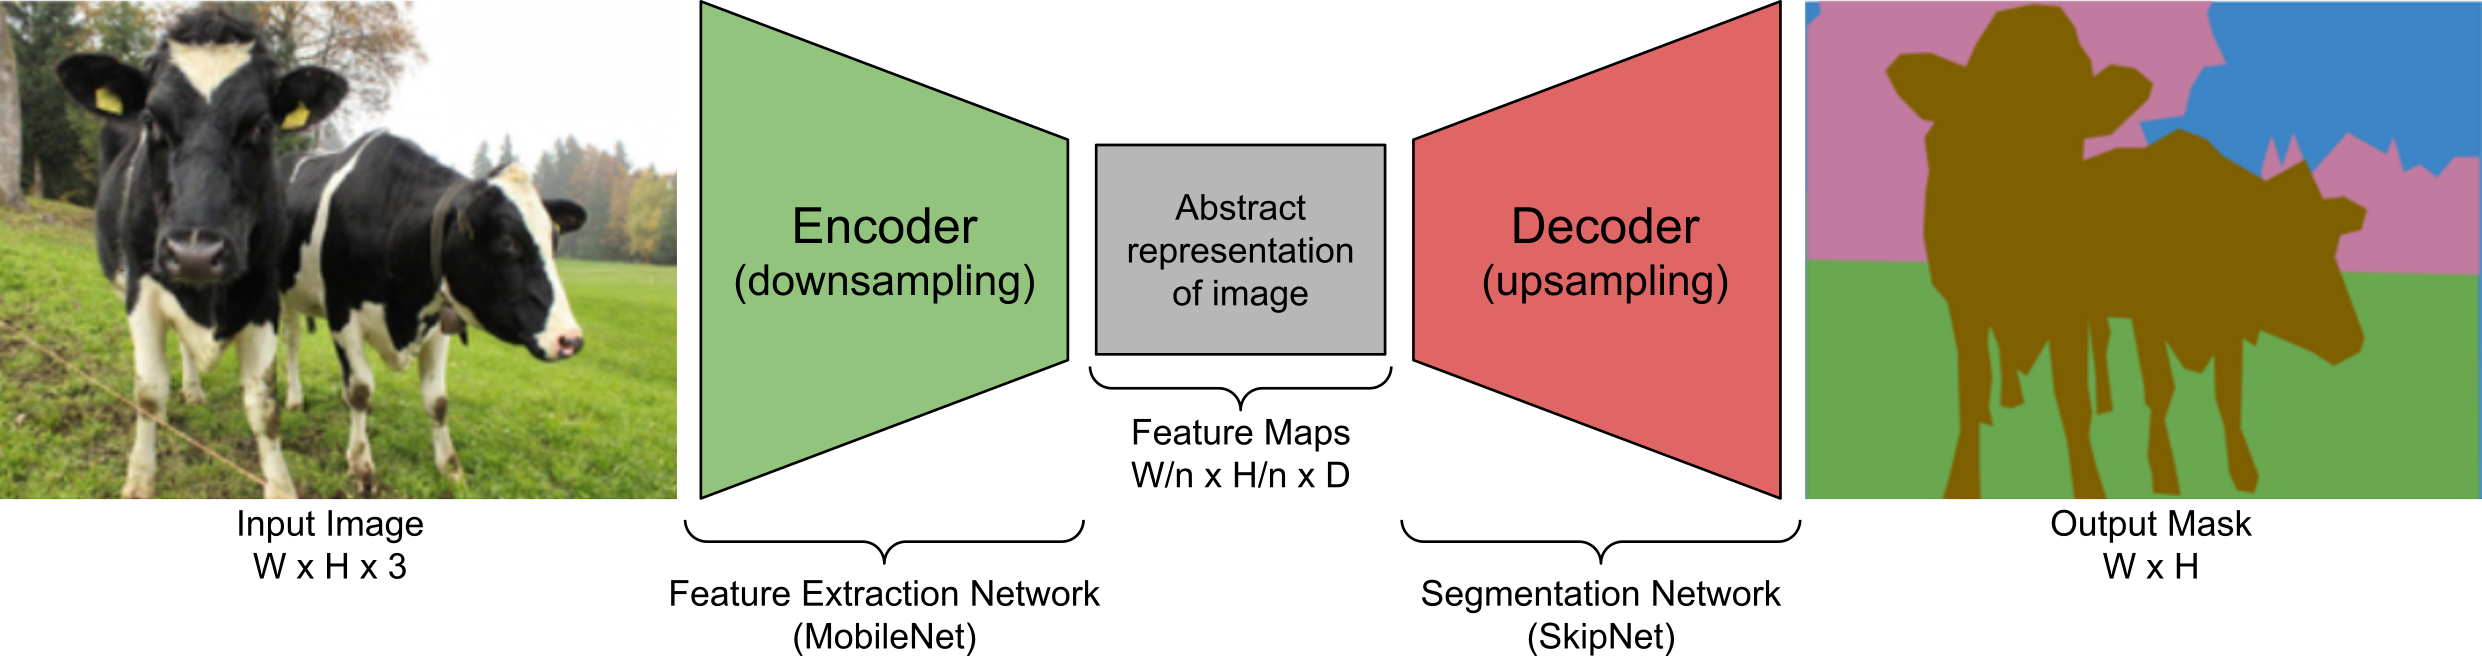
\includegraphics[width=12cm]{figures/FCN.png}
	\caption{Esquema de la arquitectura de red utilizada en este trabajo, basada en la FCN propuesta por \citet{shelhamer2017fully}. Como encoder para la extracción de features se utiliza la red MobileNet \cite{howard2017mobilenets}, lo que produce features maps con un factor de downsampling n=32. Como decoder para la producción  del mapa de segmentación se utiliza la red SkipNet \cite{siam2018rtseg}, implementando las variantes 32s, 16s y 8s.}
	\label{fig:FiguraX}
\end{figure}

Por otra parte, para recuperar la información espacial de grano fino perdida inherentemente en las capas de convolución del encoder, a menudo se utilizan conexiones que sobrepasan al menos una capa de la red llamadas \emph{skip connections}. En estas arquitecturas se utilizan para transferir información espacial local desde las capas internas del encoder directamente a la entrada del decoder. En general, estas conexiones mejoran los resultados de segmentación, ya que las skip connections mitigan la pérdida de información espacial permitiendo al decoder ver la ’’big picture’’, aunque su impacto puede variar según la skip architecture que se proponga. En \citep{long2015fully, shelhamer2017fully} se proponen tres skip architectures, que difieren en la forma en la que se implementa el decoder para realizar el upsampling y obtener el mapa de segmentación: la 32s toma los features maps y aplica una transposed convolution con factor de upsampling igual a 32, sin establecer skip connections; la 16s aplica una transposed convolution con factor de upsampling 2 a los features maps y la combina mediante una operación de suma con la capa interior del encoder del mismo tamaño (i.e. establece una skip connection), y al resultado le aplica finalmente una transposed convolution con factor de upsampling igual 16; y la 8s toma el resultado de la operación de suma de la arquitectura anterior y le aplica una transposed convolution con factor de upsampling 2, y al resultado le aplica finalmente una transposed convolution con factor de upsampling igual 8. Dado que los resultados reportados en la literatura no son concluyentes respecto a que arquitectura es mejor, en los experimentos de este trabajo se consideran las tres.


\begin{figure}
    \centering
    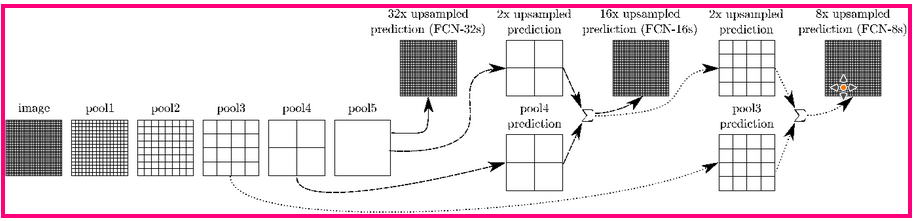
\includegraphics[width=12cm]{figures/FCN2.png}
    \caption{Dejo esta imagen de referencia para que se entienda lo que expliqué más arriba.}
    \label{fig:dataset}
\end{figure}

Estas arquitecturas han alcanzado excelentes resultados en muchas aplicaciones de segmentación de imágenes \cite{litjens2017survey, garcia2018survey, kaymak2019brief}. Sin embargo, estas redes conllevan una importante carga de recursos computacionales. Con esto en mente, en este trabajo se reemplazó el encoder VGG \cite{Simonyan2015VeryDC} propuesto originalmente por Long para las FCN, por la red MobileNet \cite{howard2017mobilenets}, una red que se destaca por tener tan solo 4.2 millones de parámetros frente a los 138 millones de parámetros de VGG, permitiendo que el proceso de entrenamiento y testeo sea considerablemente más rápido y con requerimientos de memoria muy inferiores. El uso de MobileNet como encoder en las FCN de \citep{long2015fully, shelhamer2017fully} no es novedoso, sino que ha sido ya propuesto para la arquitectura 8s por \citet{siam2018rtseg} en su arquitectura SkipNet. Técnicamente la propuesta de \citet{siam2018rtseg} es sumamente sencilla, por lo que nos atrevemos aquí a extenderla a las arquitecturas 16s y 32s propuestas originalmente por \citep{long2015fully, shelhamer2017fully}.

\subsubsection{Sliding Windows y Clasificador de patches (SW-C)}


Para contrastar los resultados alcanzados por la FCN-MN, se propone una aplicación casi directa del enfoque propuesto por \citet{perez2017image} para clasificación de imágenes de yema, el cual se utiliza como componente dentro de un mecanismo sencillo para detección de yemas por sliding windows descrito brevemente en \citet{perez2017image}. 

Este enfoque opera en tres pasos: (i) aplica el algoritmo de sliding windows sobre una imagen para extraer patches (sub-imágenes o regiones rectangulares); (ii) clasifica (todos los píxeles de) cada patch en yema o no-yema mediante el algoritmo presentado en \citet{perez2017image}; y (iii) produce la máscara de segmentación final mediante un esquema de votación. A continuación se dan los detalles de cada paso.

Las técnicas sliding windows comprenden una familia de algoritmos ampliamente utilizados en el pasado como parte de diversos enfoques para localización de objetos con bounding boxes \cite{divvala2009empirical, wang2009hog, chum2007exemplar, ferrari2007groups, dalal2005histograms, rowley1996human}. En estos algoritmos, cada imagen es escaneada densamente desde un extremo de la imagen (e.g. esquina superior izquierda) hasta el otro extremo (e.g. esquina inferior derecha) mediante una ventana deslizante rectangular en diferentes escalas y diferentes desplazamientos, extrayendo sub-imágenes o patches de la imagen original. En este trabajo, se definen 10 tamaños de ventana de igual alto y ancho, a saber 100, 200, 300, 400, 500, 600, 700, 800, 900 y 1000 píxeles, con un desplazamiento horizontal del $50\%$ el ancho de la ventana y un desplazamiento vertical del $50\%$ el alto de la ventana, lo que produce una superposición del $50\%$ entre parches contiguos. Estos valores se eligen sobre la base del análisis de robustez del clasificador que presenta \citet{perez2017image} para la geometría de la ventana. Este análisis muestra que el clasificador (explicado en la sección \ref{swtrain}) es robusto para los patches que contienen al menos $60\%$ de los píxeles de una yema, y estos deben cubrir al menos el $20\%$ del patch. Los autores argumentan que el clasificador propuesto (explicado a continuación) es lo suficientemente robusto al tamaño y posición de la ventana para realizar la detección de yemas de vid en los típicos algoritmos de sliding-windows. un algoritmo de detección por sliding-windows podría proponer fácilmente un esquema para elegir el tamaño y el desplazamiento de la ventana que garantice que en algún punto del escaneo la ventana satisface los requerimientos de robustez. Sin embargo no se dan detalles de cómo implementarlo, por lo que en este trabajo solo nos limitamos a reportar resultados para tamaños fijos de ventana y desplazamiento explicados. Dado que las yemas del corpus tienen un diámetro en píxeles variable (correspondientes a parches que varían de 100×100 a 1600×1600 píxeles aproximadamente) no todos los tamaños de ventana podrán satisfacer los requerimientos de robustez para todos los patches, pero los resultados todavía pueden ser útiles a los efectos de realizar la comparación con el enfoque FCN-MN. Con base en estos resultados, y el hecho de que las yemas del corpus tienen un diámetro en píxeles variable (correspondientes a parches que varían de 100×100 a 1600×1600 píxeles aproximadamente), se considera que los valores de ventana establecidos en este trabajo deberían producir una cobertura de yemas dentro de los valores aceptados en el análisis de robustez. 

El segundo paso de este enfoque consiste en determinar si un patch es de clase yema o no-yema. El clasificador de \citet{perez2017image} toma los patches producidos por el sliding windows y para cada uno realiza las siguiente operaciones: (i) computa features visuales de bajo nivel mediante el algoritmo \emph{Scale Invariant Feature Transform} (SIFT) \cite{lowe2004distinctive}; (ii) construye un descriptor de alto nivel para cada patch empleando el algoritmo \emph{Bag of Features} (BoF) \cite{csurka2004visual} sobre los features SIFT del paso anterior; y (iii) determina la clase de cada patch usando el descriptor BoF sobre un clasificador construido mediante el algoritmo \emph{Support Vectors Machine} \cite{vapnik2013nature}. Los detalles del entrenamiento de este clasificador se posponen hasta la sección \ref{swtrain} (Entrenamiento SW-C).

Finalmente, el tercer paso del enfoque consiste en construir la máscara binaria donde se encuentran etiquetados los píxeles que pertenecen a la clase yema y no-yema. Esta máscara es construida a través de un esquema de votación donde cada píxel suma un voto por cada patch que lo contiene clasificado como yema, el cual podría ser de un máximo de 4 para algunos píxeles debido a que el deslizamiento propuesto entre patches presenta solapamiento tanto horizontal como vertical. Luego, se establece un umbral de votos mínimos $\nu$ que puede tomar los valores del 1 al 4, de tal manera que los píxeles con una cantidad de votos igual o mayor a $\nu$ son clasificados como yema, caso contrario se clasifican como no-yema.

\subsection{Colección de imágenes}

La colección de imágenes utilizada en este estudio consiste en el mismo corpus de imágenes utilizadas originalmente en \citet{perez2017image}, el cual se ha descargado de la URL indicada por los autores http://dharma.frm.utn.edu.ar/vise/bc. 

Estas imágenes fueron capturadas en viñedos del Departamento de Ciencias Agrícolas, Universidad Nacional de Cuyo, Mendoza, Argentina, y en viñedos del Instituto Nacional de Tecnología Agropecuaria, sucursal de Luján de Cuyo, Mendoza, Argentina. Los dispositivos de captura fueron tres: (1) cámara compacta Nikon Coolpix P530; (2) cámara compacta Samsung NX1000; y (3) cámara móvil Samsung SM-G920I. Todas las imágenes fueron capturadas en formato JPEG con resoluciones  de 12Mpx a 20Mpx, y en condiciones normales de campo, sin alterar la escena con elementos artificiales y manteniendo las condiciones de iluminación natural. En algunos casos, las imágenes se tomaron también con flash para mayor variabilidad. En total, se capturaron 760 imágenes que contenían uno o más yemas por imagen, junto con otros elementos de los viñedos y su entorno natural, como tallos, hojas, troncos, sarmientos, zarcillos, alambres, tierra, otras plantas, cielo y más. Las fotos fueron capturadas entre las 10 am y las 4 pm, en varias campañas entre el 10 de julio y el 24 de septiembre de 2015 (segunda mitad del invierno de Argentina), cuando las hojas de la planta están secas o caídas, pero antes de que comenzaran a brotar nuevamente. De las 760 imágenes de esta colección, se seleccionaron las 698 imágenes que contenían sólo una yema. En este conjunto de imágenes el diámetro de las yemas varía de 100 a 1600 píxeles. Cada imagen está acompañada de una máscara con el ground truth, es decir la segmentación manual de la yema que contiene . 

Este corpus de 698 imágenes y sus máscaras fueron empleadas durante el entrenamiento y evaluación de los dos enfoques propuestos. Para esto, el corpus de imágenes se separó en dos subconjuntos disjuntos: el \emph{trainset} con el $80\%$ de las imágenes y el \emph{testset} con el restante $20\%$. Esto resultó en un trainset de 558 imágenes y un testset de 140 imágenes, ambos con sus respectivas máscaras ground truth. De esta manera, los dos enfoques propuestos utilizan exactamente las mismas 558 imágenes durante el entrenamiento, y las mismas 140 imágenes durante la evaluación.

\subsection{Entrenamiento de los modelos} 

En esta sección se dan los detalles del proceso de entrenamiento para cada enfoque empleando las 558 imágenes del trainset.

\subsubsection{Entrenamiento enfoque SW-C} 
\label{swtrain}

La etapa de entrenamiento para este enfoque se realiza de la misma manera que para el workflow original propuesto en \citet{perez2017image}. Esto implica entrenar un clasificador binario para que aprenda el concepto de yema y no-yema a partir de un corpus de patches rectangulares que contienen o no una yema. Durante el entrenamiento, los patches yema deben ser regiones que circunscriben perfectamente la yema (ver FIGURA). Los patches no-yema deben ser regiones que no contienen ni un solo píxel de yema (ver FIGURA). Por lo tanto, para construir el corpus de patches, se procesaron las 558 imágenes y sus máscaras siguiendo el mismo protocolo que en \citet{perez2017image}, obteniendo un total de 558 patches que circunscriben a cada yema (existe una por imagen) y más de $25000$ patches no-yema (el área no-yema es mucho mayor al área que ocupa una yema en la imagen). El tamaño de estos patches es variable, con resoluciones entre $0.1$ y $2.6$ megapíxeles aproximadamente (patches de $100 \times 100$ a $1600 \times 1600$ píxeles).

A partir de este corpus de patches, se creó un trainset de patches balanceado, i.e. con 558 patches de cada clase, donde los patches no-yema fueron tomados al azar entre miles de patches. El entrenamiento se realizó tal como se detalla en el pipeline propuesto en \citet{perez2017image}: (i) se extrajeron descriptores SIFT todos los patches del trainset; (ii) se aplicó BoF con tamaño de vocabulario igual a 25, dado que fue el modelo con mejores resultados según los autores; y (iii) se entrenó el clasificador SVM sobre los descriptores BoF de cada patch, empleando un kernel \emph{Radial Basis Function}, donde el valor de los parámetros $\gamma$ y C se estableció mediante un 5-fold cross-validation sobre los mismos rangos de valores, i.e. $\gamma = \{2^{-14}, 2^{-13}, … , 2^{-7}\}$ y $C = \{2^{5}, 2^{6}, … , 2^{14}\}$.

\subsubsection{2.3.2. Entrenamiento enfoque FCN-MN.} \label{fcntrain}

Para el entrenamiento de este enfoque se utilizaron las 558 imágenes reservadas para este propósito, las mismas que se usaron para el entrenamiento del enfoque anterior. Estas imágenes presentan diferentes resoluciones, sin embargo las FCN requieren una entrada de tamaño fijo. Por esto, todas las imágenes (incluida sus máscaras) fueron escaladas a una resolución de $1024 \times 1024$ píxeles usando un método de interpolación bilinear. Dado que la cantidad de imágenes en el trainset se considera escasa, para lograr un entrenamiento robusto se usaron dos técnicas ampliamente utilizadas en la práctica: usó un enfoque de \emph{transfer learning} \cite{pan2009survey} y \emph{data augmentation} \cite{shorten2019survey}. sobre el corpus de entrenamiento. Esto implica tomar una FCN previamente entrenada sobre un gran conjunto de imágenes y transferir su conocimiento a nuestro conjunto, mucho más pequeño. 

Por lo tanto, el entrenamiento se realiza en tres etapas:

\begin{enumerate}
	\item Se inicializa la red MobileNet pre-entrenada sobre el dataset ImageNet, se modifica su decoder por uno de clasificación binaria.
	\item Se entrena la red para clasificar patches de forma análoga al entrenamiento de SVM para Sliding Windows;
	\item Se toman los pesos del encoder de la red resultante en el paso anterior y se entrenan las 3 arquitecturas de FCN sobre el corpus de entrenamiento compuesto por imágenes completas y sus correspondientes máscaras binarias augmentadas.
\end{enumerate}
%
Para el tuning FCN se realizó 4-fold cross validation por 60 epochs, variando sobre los métodos de optimización Adam ($Learning Rate = 0.001$, $beta1= 0.9$ y $beta2 = 0.999$), RMSProp ($Learning Rate = 0.001$ y $rho = 0.9$) y Stochastic Gradient Descent (Learning $Rate = 0.0001$ y $Momentum = 0.9$) y Dropout ($\{0.001, 0.5\}$), donde los parámetros para RMSProp y Adam corresponden a los sugeridos por los autores \cite{ruder2018gradientdescent}. El preprocesamiento aplicado en el paso 3 fue un escalado de las imágenes a tamaño $1024 \times 1024$px (debido a restricciones en capacidad de cómputo), y un scaling en los valores de intensidad de los píxeles RGB [0,255] a [-1, 1].

\begin{table}[]
	\begin{tabular}{ll}
		\hline
		\textbf{Parámetros} & \textbf{Promedio IoU} \\ \hline
		RMSProp y Dropout = 0.001 & 0.44253 \\
		RMSProp y Dropout = 0.5 & 0.3117 \\
		Adam y Dropout = 0.001 & 0.240277 \\
		Adam y Dropout = 0.5 & 0.315714 \\
		SGD y dropout = 0.001 & 0.000886 \\
		SGD y dropout = 0.5 & 0.00151 \\ \hline
	\end{tabular}
	\caption{Promedio de IoU sobre las 3 variantes para cada combinación de parámetros.}
	\label{tab:TablaX}
\end{table}

Observamos en la Tabla \ref{tab:TablaX} que la combinación de parámetros con la que alcanzamos mayor IoU promedio es RMSProp con dropout de $0.001$. Se procedió a entrenar las 3 variantes con estos parámetros sobre el conjunto de entrenamiento completo por 200 epochs. Las augmentations realizadas sobre el conjunto de entrenamiento se llevaron a cabo con los siguientes parámetros (rangos con probabilidad uniforme): Rotación de hasta $45\degree$, traslación horizontal de hasta el $40\%$ con probabilidad uniforme, traslación vertical de hasta el $40\%$ con probabilidad uniforme, Shear de $10\%$, Zoom de hasta $30\%$, $0.5$ de probabilidad flip horizontal y $0.5$ de probabilidad de flip vertical. 


%#######################################################################
%#######################################################################
\section{3. Resultados Experimentales} \label{results}

In this section we present a systematic evaluation of the quality of the bud detector proposed in this work. For that, we first evaluate our approach in terms of its detection capabilities, by reporting the correspondence between the connected components of the mask produced by the detector and the mask of the actual buds. Then, we refine the evaluation by reporting  the quality of the segmentation for those connected components that correctly detected a bud. We start in the following section by defining the metrics used to validate both detection and segmentation, and then proceed to compare the results of applying those metrics to the masks produced by our FCN approach against those of the scanning windows approach of cite{perez2017image} (c.f. Section~\ref{sec:XXX}), over all 140 images of the test corpus.
%
\subsection{Métricas de Performance}

We considered metrics for each of the two main operations: detection and segmentation discussed in detail in the following two subsections.



\subsubsection{Detection metric Métricas para evaluación de individualización. }

Detection of buds is the result of the post-processing of the segmented mask into connected components of its positive pixels. This process may result in several types of errors whose analysis is complicated when there is an unknown number of true buds in the scene (see \cite{oguz2017dice} for a thorough analysis and description of all possible detection metrics, for instance, ambiguous detections when a connected component overlaps more than one true bud). To avoid confusing or an overly complex analysis our image corpus contains a single bud per image, resulting in the following subset of possible cases:

\begin{itemize}
	\item \emph{Correct Detection} (\textbf{CD}) is the best case, when the detected mask presents a single connected component, and this connected component overlaps with the true bud of the image. This would correspond with a \emph{true positive} situation.
	\item \emph{Split} (\textbf{S}) occurs when there is more than one detection per bud, which happens  when the mask contains multiple connected components, all of which overlaps the true bud. 
	\item \emph{False Alarm} (\textbf{FA}), equivalent to a \emph{false positive} situation, corresponds to segmented connected components not overlapping with the true bud.
	\item \emph{Detection Failure} (\textbf{DF}) , equivalent to a \emph{false negative}, is when the detection mask presents no connected components.
\end{itemize}

All four of these cases categorize buds (or images, as all test images contain a single bud), and are mutually exclusive, that is, no bud can satisfy any two (or more) of these definitions simultaneously. This suggests that a simple performance metric would be the counts of the number of images for each category, with the best case consisting in all images in the CD category. This would even allow a normalization. However, it results in a better analysis and comparison of detection failures to quantify the actual number of false alarms per image. We thus report the categories CD, S and DF as the number of images in those categories, and category FA as the number of connected components satisfying its condition.
To simplify the reporting, we further combine these quantities in two steps. First, we count splits as (a single) true positive together with the correct detection and then report the percentage of all true positives that resulted in splits. This allows us to combine these counts  in the well known precision and recall metrics, named hereon \emph{detection-precision} and \emph{detection-recall}, computed as:

\begin{equation}
detection \mbox{-} precision = \frac{true\ positives}{true\ positives+false\ positives} \\
= \frac{CD+S}{CD+S+FA}
\label{eq:detection-precision}
\end{equation}

\begin{equation}
detection \mbox{-} recall = \frac{true\ positives}{true\ positives+false\ negatives} \\
= \frac{CD+S}{CD+S+DF}
\label{eq:detection-recall}
\end{equation}

Finally, based on these quantities, one could also compute the \textbf{F1-measure}, the harmonic average of precision and recall: \( 2 \times \frac{precision \times recall}{precision + recall}\).

\subsubsection{Segmentation metric}

Detection metrics, although informative, relies on overlap between the detected and true bud, regardless of how minimal the overlap. This could miss several possible pixelwise detection errors, resulting in rather coarse comparisons between competing detection algorithms. For instance, a correct detection could present a very small overlap with the true bud, with many or even a majority of the true bud’s pixels missing (i.e., several \emph{false negatives} pixels), or could be erroneously reporting several pixels as bud pixels (i.e., several \emph{false positives} pixels). Clearly, the best case scenario would be a case of correct detection with no false negatives or positives, that visually would correspond to a perfect overlap of the detected connected component and the true bud.  A pixel wise comparison of the masks could also help assess the quality of the splits. The best split, for instance, would be one completely enclosed within the true mask, i.e., with none of its connected components presenting false positives; while covering as much of the true bud mask as possible, i.e., presenting just enough false negatives to disconnect its components. Finally, a false alarm case, clearly presenting only false positive pixels, could be further assessed by the number of (false positive) pixels in its components. 

The community has proposed several metrics to quantify  segmentation errors. The most obvious ones are those that count the number of pixels in each category, resulting in real number metrics running from 0 to 1, that report the \emph{fraction} of the whole image corresponding to \emph{true positives}, denoted $TPF$; \emph{false positives},  denoted $FPF$;  and \emph{false negatives}, denoted $FNF$. Also, to simply the analysis, one could combine these quantities into the well known (pixel wise) \emph{precision}  and \emph{recall}, computed as $TPF / (TPF + FPF)$  and $TPF / (TPF + FNF)$, respectively. Another combination of these quantities, useful to assess the relative size of the false positives, is the \emph{false-positive-rate}, computed as $FPF/(FPF + TNF)$, or simply $FPF / NF$, where the latter is the fraction of negatives, that is, all except the true bud pixels. But even these two quantities can be simplified into a single quantity in two different ways. One is the weighted harmonic mean of precision and recall, the well-known \emph{F-measure}, formally $2 \times precision \times recall / (precision + recall)$, proposed independently for segmentation overlap measurement by (Dice 1945); and the other is the  Jaccard’s \emph{intersection-over-union} (Jaccard 1912), equivalent to $TPF / (TPF+FPF+FNF)$. 

With these metrics, one could quantify the refinements discussed in the first paragraph above, by simply applying them, no to the whole mask, but to the individual categories. For instance, reporting the mean Dice measured over all correctly detected components; or to refine the assessment of how bad is a split, one could report the mean Dice measure to all components of some split, or the mean Dice measure over all split components of all split images. Finally, one could report the mean false-positive-rate over all images to assess the gravity of the false alarm components produced by some algorithm.

\subsection{Resultados Sistemáticos}

We proceed now to assess the validity of our main hypothesis, namely, that FCN is a better detector than its SW counterpart, through a sequence of comparisons of increasing refinement by reporting results for the detection metrics first, to then report comparisons in terms of segmentation metrics. 

\subsubsection{Detection metrics comparison of FCN and SW}

We start by reporting the comparison of detection-precision and detection-recall, to then analyze how many of the true positives involved are indeed splits.  Figure \ref{fig:1.1.1} shows a precision-recall scatterplot, with results for FCN (SW) in black (white) dots, each representing the detection-precision and detection-recall computed over all images in the test set,  obtained for detection executed by a model trained for one specific  configuration of hyperparameters. For FCN, these hyperparameters would be the architecture, with values 8s, 16s and 32s, and threshold $\tau$ with values in  $\{0.1, 0.2, \ldots, 0.9\}$, resulting in a total of 27 black dots; while for SW these hyperparameters would be the (squared) patch sizes with values in $\{100, 200, \ldots, 1000\}$ and voting threshold with values in $\{1, 2, 3, 4\}$, for a total of a total of 40 white dots. 

\begin{figure}
	\centering
	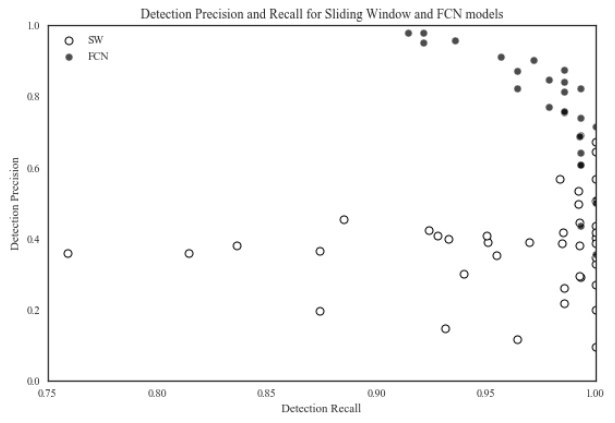
\includegraphics[width=12cm]{figures/detection-scatter-plot.png}
	\caption{Precision-Recall scatterplots reporting the results for FCN and SW with black and white dots, respectively. Each dot represents the detection-precision and detection-recall computed over all images of the tests, for some particular  configurations of hyperparameters. For FCN, these would be the architecture, with values 8s, 16s and 32s, and threshold $\tau = \{0.1, 0.2, \ldots, 0.9\}$,  for a total of 27 black dots; while for SW these would be the patch sizes  $\{100, 200, \ldots, 1000\}$ and voting thresholds $\{1, 2, 3, 4\}$, for a total of a total of 40 white dots.}
	\label{fig:detection-scatter-plot}
\end{figure}

The graph shows that both cases accumulate several dots at values of maximum recall, expected for cases that favor the positive pixels. Indeed, for SW this is clearly the case for voting threshold of 1 (squared dots), for which recall is $1.0$ in all cases, while for larger voting thresholds recall grows with the patch sizes (dots of larger size).

The other important conclusion of the figure is that FCN shows a clear and undisputed improvements over SW, with larger detection-precisions over the majority of scenarios, resulting in a larger area under the PR curve. Also, table XXX shows the F1-measure values for each algorithm, sorted in decreasing order,  showing that the first $Y\%$ of the FCN cases has larger F1-measure than all of SW, and only $Z\%$ ....

As mentioned earlier, some of the correctly detected components may be splits. These splits are troublesome for scenarios in which there is no prior knowledge of the number of true buds in the scene: a split is the detection of a single bud, or the detection of several buds? All we can do here is to assess the tendency of our algorithms to produce splits.  We thus computed the number of splits produced (over all images in the test set) produced by each of the models obtained for the different configurations of the hyperparameters. Figure \ref{fig:number-of-split} shows a summary of these results in the form of a histogram, with bins representing the mean number, over all images, of splitted components produced by a model, and the bars for that bin representing the proportion of models that resulted in a mean number of splits indicated by the bin’s label, with  black and white bars for FCN and SW, respectively. For instance, the first bin indicates that approximately $54\%$ of the FCN models and approximately $62\%$ of the sliding window models resulted in a mean number of splits (over all images in the test set) of less than $5$. For the second bin, around $25\%$ of the models produced by FCN versus approximately $4\%$ of the models produced by SW resulted in a mean number of splits between $5$ and $10$. Overall, FCN distribution is slightly more concentrated in the lower number of splits than the SW distribution, but in general both algorithms compare fairly, with no clear contender when compared on the average number of splits they produce. 

\begin{figure}
	\centering
	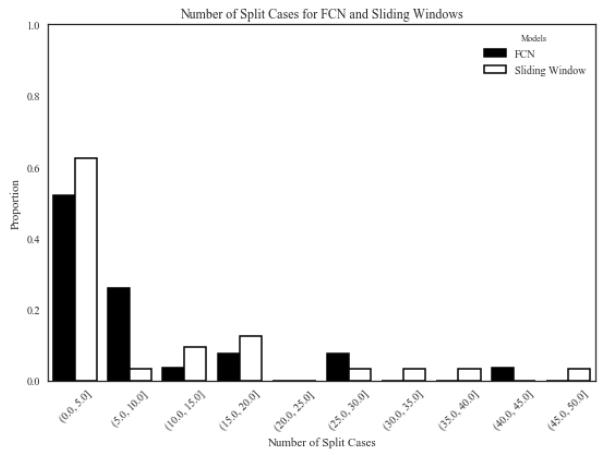
\includegraphics[width=12cm]{figures/number-of-split.png}
	\caption{Histogram reporting the distribution of the mean number of splits per model for FCN and SW in black and white bars, respectively. Each bar represents the normalized frequency among all models ($27$ for FCN, $9$ thresholds and $3$ architectures;  and $40$ for SW, with $10$ window sizes and $4$ voting thresholds) that contains the number of splits of the bar’s position. For instance, the first (from left to right) white bar indicates that almost $14\%$ out of the $40$ SW models contains between $0$ to $5$ splits. }
	\label{fig:number-of-split}
\end{figure}

\subsubsection{Segmentation metrics comparison of FCN and SW}

In this section we analyze comparisons of the two methods, FCN and SW, with some detail on the segmentation quality of each method. We start in the following subsection reporting the segmentation quality of the true positives, showing results of the segmentation metrics \emph{precision} and \emph{recall} for the \emph{correct detections} and \emph{splits}. Then, in Section UUU we discuss segmentation metrics for the \emph{false alarm} components after introducing the \emph{normalized area} and \emph{normalized distance} metrics. 

\subsection{Section 111. Segmentation metrics for Correct Detections and Splits}


These figures show segmentation-precision versus segmentation-recall scatter plots over all models produced for each method, one per configuration of the hyperparameters (architecture and detection threshold for FCN, and window size and voting parameter for SW), with one dot per configuration/model. Each dot represents the mean precision and mean recall obtained by its corresponding model over all images in the test set. 
Figures XXX(a) and XXX(b) show segmentation precision-recall scatterplots for \emph{correct detections} and \emph{splits}, respectively. The black and white dots scatter plots correspond to results of the detection models generated by the FCN and SW algorithms, respectively, with one black (white) dot for each of the $27$ ($40$) hyperparameter configurations of FCN (SW). The position of each dot in the plot corresponds to the mean segmentation-precision and mean segmentation-recall over all images in the test set, computed over the correctly detected components of the masks produced by the algorithm and configuration associated to that dot.
In Fig XXX (a) (correctly detected), one can observe that all black dots (FCN) are clustered on the upper-right corner of the graph, enclosed by a minimum precision of approximately $0.65$ and minimum recall of approximately $0.60$; while the white dots (SW) are clustered on the lower-right corner of the graph, with maximum precisions of $0.5$ and recall ranging from approximately $0.35$ to $1.0$. Overall, both algorithms show relatively high recalls, but with FCN reaching much larger precisions. We can point to the coarse detection through squared patches of the SW method as the main cause for the low precision, as this is reduced when extra, false positives are present in the positive mask. Also, for the specific case of FCN, one can observe cases of nearly $0.9$ of both precision and recall, meaning that $90\%$ of the bud is represented by the component of the detection, and that $90\%$ of the component is representing pixels of the bud. 
Fig XXX (b) shows results for the splitted detections, where the segmented precision and recall were computed over the union of all components in the split. This represents the interpretation that all components that touch a bud correspond to a single detection of the bud. Again, we can see some configurations for FCN reaching precisions over $90\%$, meaning  that the components of the splits are $90\%$ over the bud; and a recall of almost $80\%$, meaning that $80\%$ of the bud has been covered by the combination of all components of the split. Also, one can observe the overwhelming improvements of FCN over SW, with all (but one) SW cases presenting precisions under $60\%$, with the outlier showing a precision of nearly,  $70\%$, and a similar distribution of recall values.  

\begin{figure}%
	\centering
	\subfloat[]{{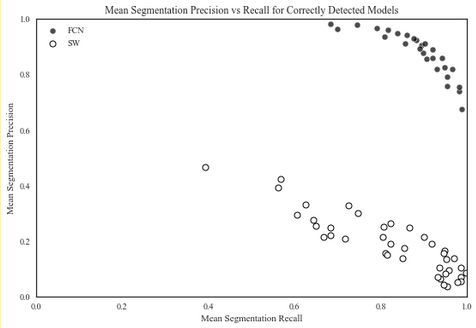
\includegraphics[width=5cm]{figures/mean-precision-recall-CD.png} }}%
	\label{fig:mean-precision-recall-a}
	\qquad
	\subfloat[]{{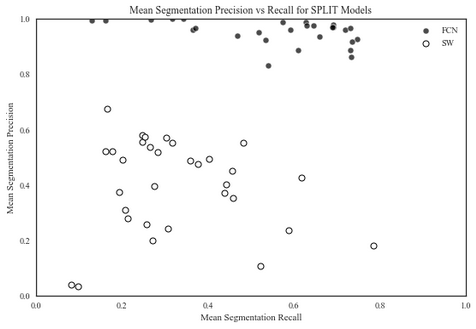
\includegraphics[width=5cm]{figures/mean-precision-recall-S.png} }}%
	\label{fig:mean-precision-recall-b}
	\caption{Segmentation Precision-Recall scatterplots reporting the results for FCN and SW in black and white, respectively, with dots representing the average of segmentation precision and segmentation recall over all images in the test set, with one dot per configuration of hyperparameters (27 for FCN, 9 thresholds and 3 architectures;  and 40 for SW, with 10 window sizes and 4 voting thresholds). In (a), the averages were computed over the segmentation precision and recall of the correctly detected components, while in (b), the averages were computed  over the segmentation precision and recall of the split components.   Standar deviations.}%
	\label{fig:mean-precision-recall}%
\end{figure}


To complete these figures, we report in Table XX the detection-precision, detection-recall, the F1 detection measure computed from them, as well as the segmentation-precision and segmentation-recall with their corresponding F1 segmentation measure which is the Dice measure, for all 27 configurations of FCN (first row) and all 40 configurations of SW (second row). The best among FCN and the best among all SW has been marked in bold. From this table, one can see that...


\begin{table}[]
	\tiny
	\centering
	\begin{adjustbox}{angle=90}
		\begin{tabular}{lllllllllllll}
			\hline
			\multicolumn{1}{|l|}{\textbf{}} & \multicolumn{4}{l|}{\textbf{Detection}} & \multicolumn{3}{l|}{\textbf{Segmentation-CD [mean (sd)]}} & \multicolumn{3}{l|}{\textbf{Segmentation-S [mean (sd)]}} & \multicolumn{2}{l|}{\textbf{FA [mean (sd)]}} \\ \hline
			\multicolumn{1}{|l|}{\textbf{Model}} & \multicolumn{1}{l|}{\textbf{Prec}} & \multicolumn{1}{l|}{\textbf{Rec}} & \multicolumn{1}{l|}{\textbf{F1}} & \multicolumn{1}{l|}{\textbf{S\#}} & \multicolumn{1}{l|}{\textbf{Prec}} & \multicolumn{1}{l|}{\textbf{Rec}} & \multicolumn{1}{l|}{\textbf{Dice}} & \multicolumn{1}{l|}{\textbf{Prec}} & \multicolumn{1}{l|}{\textbf{Rec}} & \multicolumn{1}{l|}{\textbf{Dice}} & \multicolumn{1}{l|}{\textbf{Relat Area}} & \multicolumn{1}{l|}{\textbf{Norm Dist}} \\ \hline
			$FCN_{8s}^{0.5}$ & 75,4 & 98,6 & 85,4 & 2 & 91,0 (11,3) & 90,2 (11,7) & \cellcolor[HTML]{81D41A}\textbf{89,6 (10,3)} & 96,6 (2,2) & 73,1 (17,6) & \cellcolor[HTML]{81D41A}\textbf{82,1 (10,2)} & 0,26 (0,69) & 3,72 (4,64) \\
			$FCN_{8s}^{0.9}$ & 90,1 & 97,1 & 93,5 & 8 & \cellcolor[HTML]{81D41A}\textbf{98,1 (6,0)} & 68,3 (21,1) & 77,9 (19,6) & 98,7 (3,0) & 57,4 (18,4) & 70,8 (13,6) & 0,24 (0,5) & 3,8 (5,66) \\
			$FCN_{16s}^{0.1}$ & 71,3 & \cellcolor[HTML]{81D41A}\textbf{100} & 83,2 & 6 & 75,7 (13,1) & 95,4 (14,7) & 83,1 (13,5) & 83,1 (8,9) & 54,1 (21,9) & 61,9 (17,5) & 0,12 (0,44) & 5,27 (6,53) \\
			$FCN_{16s}^{0.4}$ & 87,0 & 96,4 & 91,5 & 1 & 87,7 (12,1) & 89,8 (18,2) & 87,0 (15,6) & 96,7 (0,0) & 37,0 (0,0) & 53,5 (0,0) & \cellcolor[HTML]{81D41A}\textbf{0,04 (0,09)} & 3,8 (5,08) \\
			$FCN_{16s}^{0.6}$ & 95,6 & 93,6 & 94,6 & 3 & 92,2 (8,7) & 88,2 (13,3) & 89,1 (10,7) & 99,4 (0,6) & 16,2 (10,6) & 26,6 (16,8) & 0,08 (0,11) & \cellcolor[HTML]{81D41A}\textbf{1,1 (0,65)} \\
			$FCN_{16s}^{0.8}$ & \cellcolor[HTML]{81D41A}\textbf{97,7} & 92,1 & \cellcolor[HTML]{81D41A}\textbf{94,9} & 4 & 95,8 (7,0) & 81,6 (14,6) & 87,0 (10,7) & 99,7 (0,3) & 34,2 (32,6) & 43,9 (33,1) & 0,1 (0,12) & 1,28 (0,95) \\
			$FCN_{16s}^{0.9}$ & \cellcolor[HTML]{81D41A}\textbf{97,7} & 91,4 & 94,5 & 4 & 97,6 (5,6) & 74,5 (16,5) & 83,1 (12,8) & \cellcolor[HTML]{81D41A}\textbf{99,9 (0,1)} & 31,8 (27,9) & 41,6 (34,0) & 0,07 (0,11) & 1,33 (0,9) \\
			$FCN_{32s}^{0.1}$ & 35,4 & \cellcolor[HTML]{81D41A}\textbf{100} & 52,2 & 8 & 67,4 (14,0) & \cellcolor[HTML]{81D41A}\textbf{98,8 (3,4)} & 79,1 (11,0) & 86,0 (9,4) & 73,4 (19,6) & 77,1 (10,4) & 0,14 (0,66) & 4,62 (5,59) \\
			$FCN_{32s}^{0.2}$ & 50,9 & \cellcolor[HTML]{81D41A}\textbf{100} & 67,5 & 10 & 73,9 (13,6) & 98,1 (3,8) & 83,5 (10,1) & 92,2 (5,4) & 53,4 (25,8) & 63,6 (19,3) & 0,17 (0,55) & 4,33 (6,17) \\
			$FCN_{32s}^{0.3}$ & 49,8 & \cellcolor[HTML]{81D41A}\textbf{100} & 66,5 & 10 & 79,1 (13,2) & 95,5 (10,5) & 85,2 (11,8) & 88,5 (9,7) & 61,0 (35,1) & 65,8 (28,2) & 0,1 (0,39) & 3,68 (5,62) \\
			$FCN_{32s}^{0.6}$ & 68,5 & 99,3 & 81,1 & 16 & 89,0 (11,5) & 89,1 (11,3) & 88,1 (9,6) & 92,4 (7,7) & \cellcolor[HTML]{81D41A}\textbf{74,7 (28,1)} & 78,1 (24,0) & 0,11 (0,3) & 2,95 (4,36) \\
			$FCN_{32s}^{0.9}$ & 82,2 & 96,4 & 88,7 & \cellcolor[HTML]{81D41A}\textbf{42} & 96,2 (8,9) & 69,8 (15,9) & 79,6 (13,5) & 98,7 (3,0) & 62,8 (22,3) & 74,1 (19,4) & 0,05 (0,13) & 3,15 (4,8) \\
			$SW_{100}^{1}$ & \textbf{9,4} & \cellcolor[HTML]{E0C2CD}\textbf{100} & \textbf{17,2} & 28 & 24,6 (17,7) & 86,7 (19,5) & 33,6 (15,1) & 57,9 (28,2) & 24,8 (16,8) & 27,9 (13,8) & 1,08 (3,2) & 7,68 (6,02) \\
			$SW_{100}^{3}$ & 14,6 & 93,1 & 25,3 & 40 & 42,4 (26,4) & 56,8 (29,9) & \cellcolor[HTML]{E0C2CD}\textbf{39,9 (19,7)} & 55,5 (32,2) & 24,8 (18,1) & 26,0 (15,6) & 0,31 (0,96) & 6,45 (6,19) \\
			$SW_{100}^{4}$ & 19,5 & 87,4 & 31,9 & \cellcolor[HTML]{E0C2CD}\textbf{49} & \cellcolor[HTML]{E0C2CD}\textbf{46,5 (29,3)} & 39,2 (28,9) & 33,9 (21,1) & 49,0 (29,0) & 20,1 (13,7) & 24,1 (14,0) & \cellcolor[HTML]{E0C2CD}\textbf{0,22 (0,57)} & \cellcolor[HTML]{E0C2CD}\textbf{6,0 (6,56)} \\
			$SW_{200}^{1}$ & 20,0 & \cellcolor[HTML]{E0C2CD}\textbf{100} & 33,3 & 12 & 16,6 (12,5) & 94,9 (13,5) & 25,9 (14,2) & 49,3 (26,4) & 40,2 (17,4) & 36,8 (11,9) & 5,13 (19,3) & 7,56 (5,35) \\
			$SW_{200}^{3}$ & 26,0 & 98,6 & 41,1 & 19 & 29,9 (17,0) & 74,7 (27,3) & 38,5 (17,0) & \cellcolor[HTML]{E0C2CD}\textbf{67,5 (32,7)} & 16,5 (8,9) & 24,2 (11,9) & 1,69 (3,15) & 8,94 (6,22) \\
			$SW_{300}^{1}$ & 26,9 & \cellcolor[HTML]{E0C2CD}\textbf{100} & 42,4 & 2 & 13,7 (13,6) & 97,0 (9,6) & 21,6 (15,5) & 55,0 (11,8) & 48,1 (1,1) & \cellcolor[HTML]{E0C2CD}\textbf{50,8 (4,5)} & 7,79 (20,5) & 6,83 (4,44) \\
			$SW_{400}^{1}$ & 32,7 & \cellcolor[HTML]{E0C2CD}\textbf{100} & 49,3 & 2 & 10,5 (11,7) & 98,7 (9,3) & 17,2 (15,3) & 42,6 (10,1) & 61,9 (11,6) & 50,4 (10,9) & 11,59 (24,05) & 7,12 (4,15) \\
			$SW_{400}^{2}$ & 34,6 & \cellcolor[HTML]{E0C2CD}\textbf{100} & 51,4 & 4 & 15,6 (15,1) & 94,5 (13,3) & 23,8 (15,6) & 48,7 (27,6) & 36,0 (4,6) & 38,6 (13,1) & 9,54 (26,13) & 7,88 (4,89) \\
			$SW_{500}^{1}$ & 40,2 & \cellcolor[HTML]{E0C2CD}\textbf{100} & 57,3 & 1 & 8,40 (9,7) & \cellcolor[HTML]{E0C2CD}\textbf{99,9 (4,9)} & 14,2 (13,8) & 17,9 (0,0) & \cellcolor[HTML]{E0C2CD}\textbf{78,6 (0,0)} & 29,2 (0,0) & 17,39 (30,07) & 7,22 (4,04) \\
			$SW_{500}^{2}$ & 38,6 & \cellcolor[HTML]{E0C2CD}\textbf{100} & 55,7 & 1 & 13,5 (14,0) & 95,2 (14,5) & 21,0 (16,0) & 35,2 (0,0) & 45,9 (0,0) & 39,8 (0,0) & 17,19 (39,07) & 7,56 (4,42) \\
			$SW_{600}^{1}$ & 43,5 & \cellcolor[HTML]{E0C2CD}\textbf{100,0} & 60,6 & 0 & 6,9 (7,8) & 98,5 (10,7) & 12,0 (12,0) & nan (nan) & nan (nan) & nan (nan) & 25,48 (48,45) & 7,72 (4,3) \\
			$SW_{600}^{2}$ & 41,7 & \cellcolor[HTML]{E0C2CD}\textbf{100,0} & 58,8 & 1 & 10,4 (10,6) & 93,7 (18,9) & 17,2 (14,4) & 19,7 (0,0) & 27,2 (0,0) & 22,9 (0,0) & 20,41 (38,32) & 7,92 (4,38) \\
			$SW_{700}^{1}$ & 50,6 & \cellcolor[HTML]{E0C2CD}\textbf{100,0} & 67,2 & 0 & 5,6 (6,5) & 98,6 (12,0) & 9,9 (10,3) & nan (nan) & nan (nan) & nan (nan) & 31,95 (64,36) & 7,75 (4,45) \\
			$SW_{800}^{1}$ & 56,7 & \cellcolor[HTML]{E0C2CD}\textbf{100,0} & 72,4 & 0 & 5,1 (6,6) & 97,7 (11,0) & 9,0 (10,4) & nan (nan) & nan (nan) & nan (nan) & 44,53 (71,52) & 7,7 (4,06) \\
			$SW_{900}^{1}$ & 64,3 & \cellcolor[HTML]{E0C2CD}\textbf{100,0} & 78,3 & 0 & 4,2 (5,7) & 94,7 (19,0) & 7,5 (9,2) & nan (nan) & nan (nan) & nan (nan) & 48,16 (80,31) & 7,9 (4,35) \\
			$SW_{1000}^{1}$ & \cellcolor[HTML]{E0C2CD}\textbf{67,0} & \cellcolor[HTML]{E0C2CD}\textbf{100,0} & \cellcolor[HTML]{E0C2CD}\textbf{80,2} & 0 & 3,7 (4,7) & 95,3 (18,3) & 6,8 (7,9) & nan (nan) & nan (nan) & nan (nan) & 57,83 (84,87) & 7,91 (4,3) \\ \hline
		\end{tabular}
	\end{adjustbox}
	\caption{Details on the detection precision,  detection recall, and their corresponding  F1  measure for each of the 27 configurations of hyperparameters considered for FCN, i.e., the three architectures \{8s,16s, 32s\} and 9 thresholds $\tau=\{0.1,0.2,...,0.9\}$, as well as the 40 configurations considered for SW, i.e., the (squared) patch sizes  $\{100,200,...,1000\}$ and voting thresholds $\{1,2,3,4\}$; all sorted in decreasing order of F1.}

	\label{tab:TableXX}
\end{table}


The above results for segmentation report for each model the mean values for each segmentation metric over all images, difflicuting any possible understanding on what happens individually for each image/bud. We thus complement the above with reports of these metrics but for individual images. For that, we selected two models/configurations for FCN and two models/configurations for SW, corresponding to the best w.r.t. to the F1 detection measure and the best w.r.t. to the F1 segmentation measure or Dice metric. For FCN, the resulting models are those of architecture 16s and thresholds $\tau=0.8$ and $\tau=0.6$ corresponding to the one with highest F1 and the one with highest Dice, respectively. For SW, the model with highest F1 detection measure is the one with 1000px window size and voting threshold 1, whereas the one with highest Dice is the one with 500px window size and voting threshold 4. 
As above, we discriminate the results for the \emph{correctly detected} and \emph{splitted} components, shown in Figures ZZZ (a) and (b),  respectively. These figures show four scatterplots each, one for each of the four cases, with black (white) elements representing the results for the two hyperparameter configurations chosen for FCN (SW); specifically, the black circles for the FCN with architecture 16s and threshold $\tau=0.8$,  the black squares for the  FCN with architecture 16s and threshold $\tau=0.6$, the white circles for the SW with patch size of $1000$ and voting $1$, and white squares for the SW with patch size $500$ and voting threshold $4$. Here, there is one point in the scatter plot per image in the test set, whose coordinates correspond to its segmentation precision and recall. In Figure ZZZ(a), the precision and recall is computed over the \emph{correctly detected} component of the image (w.r.t. the mask of the true bud); while in Figure ZZZ(b),  the precision and recall is computed over the union mask of all \emph{splitted} components.
Figure ZZZ (a) shows a scatterplot for the segmentation precision versus segmentation recall computed for each \emph{correctly detected} component in the test set of images; with squared and circled dots representing cases of FCN and SW, respectively, with black dots representing the case of higher F1 and hollow dot representing the case of secondly ranked F1, e.g., black circles represent SW with second to best detection F1 measure. Similarly, Figure ZZZ (b)  shows the precision-recall scatterplot for the split components, where here, a dot represents the segmentation precision and recall of a single component of the split, not the precision and recall of the joint split as before. 
These results show the same trend shown for the plots over configurations, where FCN (black squares and circles) overwhelmingly improves over SW (white squares and circles). For the correctly detected (Figure ZZZ (a)),  one can see an even more pronounced clustering of FCN (black) dots on the upper-right corner with precisions much higher than those of SW (white), with some outliers of small recall, or small precision; clearly those responsible for lowering the mean precision and recall reported for this particular configuration in Figure XXX. Also, one can observe two different behaviours for the white dots (SW), where both present recall values over the whole range, but the white circles (SW with highest Dice) show considerably higher precisions, with cases over $0.6$.  
The split case, Fig. ZZZ (b),  shows some interesting conclusions as well. First we note that the case of SW with window size of 1000px (white circle) has no points in the scatter plot, as a result of no splits for that case. This is expected given the large size of the patch. Also, one can notice that all split components of both cases of FCN (black squares and black circles)  have precision of practically $1.0$, while the (single) case of SW presents several split components with small precision. Large precision, regardless of the recall, shows these splits are correct detection that has been splitted, that is, components that are entirely within the true bud but that are not connected among themselves. 

\begin{figure}%
	\centering
	\subfloat[]{{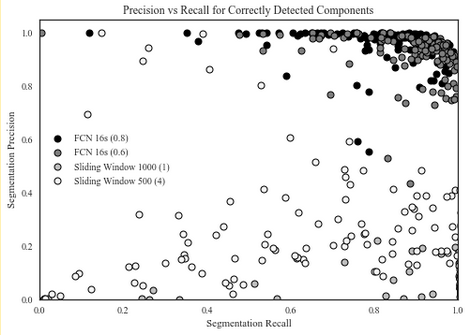
\includegraphics[width=5cm]{figures/precision-recall-CD.png} }}%
	\label{fig:precision-recall-a}
	\qquad
	\subfloat[]{{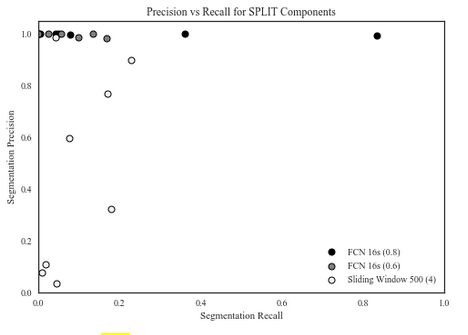
\includegraphics[width=5cm]{figures/precision-recall-S.png} }}%
	\label{fig:precision-recall-b}
	\caption{ (a) Correctly detected y (b) Splits.}%
	\label{fig:precision-recall}%
\end{figure}

\subsection{Reports for False Alarms} 
\label{sec:falsealarmsrep}

Segmentation results for correct detection and splits allowed us to further assess the quality of the detections. However, as shown by the detection precision and recall results above, there is no lack of false detections, the false positive components we called false alarms. For instance, in their best versions, $2.3\%$ of all components produced by the FCN with threshold $0.8$ and architecture 16s are false alarms, increasing to $33\%$ for the case of SW with voting threshold 1 and windows size 1000px.  These percentages, however, do not tell us how bad these false alarms are. Whether they are large or small, or whether they are located nearby the true bud (appearing more as splits than false alarms) or they are further away. 

To improve in our understanding of the detection results for false alarms, we introduce two new metrics specifically for these type of components:

\begin{itemize}
	\item \textbf{Normalized Área (NA):} the total área (i.e., number of pixels) of the component, normalized by the area of the true bud, given a sense of scale to false alarms by comparing it to the size of the (single) true bud in the image. 
	\item \textbf{Normalized Distance (ND):}  the distance between the center of mass of the false alarm component to the center of mass of the true bud, divided by the diameter of the true bud (defined as the maximum distance between any two border points of the true bud).
\end{itemize}

\begin{figure}%
	\centering
	\subfloat[]{{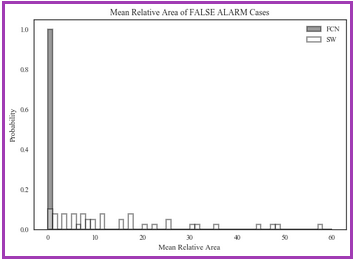
\includegraphics[width=5cm]{figures/mean-area-FA.png} }}%
	\label{fig:mean-FA-a}
	\qquad
	\subfloat[]{{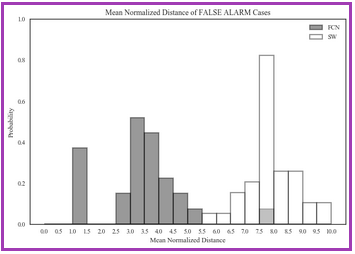
\includegraphics[width=5cm]{figures/mean-distance-FA.png} }}%
	\label{fig:mean-FA-b}
	\caption{TODO:redactar}%
	\label{fig:mean-FA}%
\end{figure}

Similarly to the correct detection and splits case, we report results for each of the $27$ models of FCN and each of the $40$ models of SW. For each model, we computed the mean NA of each false alarm component occurring on each of the images in the test set, obtaining $27$ mean NA for FCN and $40$ mean NA for SW. We then grouped the models based on similar mean NA resulting into the histogram of Figure AAA(a). One can observe, again, an overwhelming improvement of FCN over SW, where all FCN models (in black bars) resulted in small (less than $0.50$) NA (on average over all false alarmas of all images). For SW the situation is rather different, with models presenting very large false alarms, with the worst cases of sizes 60 times larger than the true bud. 
Figure AAA (b) shows a similar histogram, but grouping the mean NDs of false alarm components of each model. Again, the advantage of FCN over SW is clear, with FCN producing false alarm components at 3-4 diameters distance to the true bud (with one outlier at 7), while SW produces false alarm components at around 6 to 10 diameters of a bud.

\begin{figure}%
	\centering
	\subfloat[]{{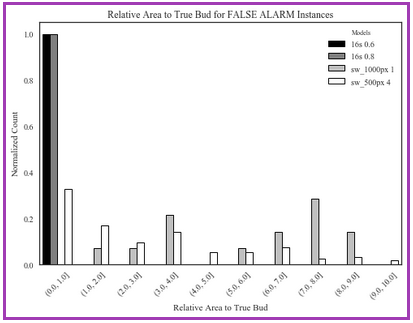
\includegraphics[width=5cm]{figures/realtive-area-truebud-FA.png} }}%
	\label{fig:truebud-FA-a}
	\qquad
	\subfloat[]{{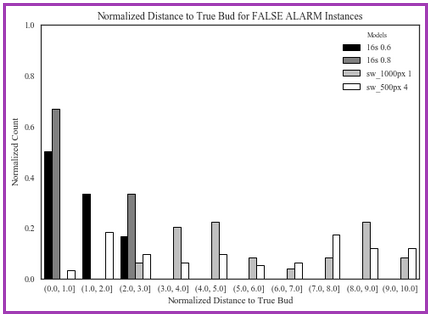
\includegraphics[width=5cm]{figures/normalized-distance-truebud-FA.png} }}%
	\label{fig:truebud-FA-b}
	\caption{Figure CCC a and b for the normalized área (NA) and distances (ND) .....}%
	\label{fig:truebud-FA}%
\end{figure}

To further understand the results at a more refined level, we repeated the analysis performed for correct detections and splits, reporting the NA and ND over individual components for the same four models selected of higher mean F1 detection measure and the one with higher mean Dice metric for both FCN and SW. Again, we group them in histograms, shown in Figures CCC (a) and (b) for NA and ND, respectively. Here, the bars represent (normalized) counts of false alarm components. It is not a surprise that these figures confirm the improvements of FCN over SW reported for the mean over images (Figure AAA). For these four models in particular, they show that all false alarm components for FCN have an area smaller than that of the bud, i.e., an NA smaller than 1.0, whereas for SW we can observe false alarm components of sizes as large as $10$ time of that of the actual bud. Figure CCC (b) shows, for these four models, that absolutely all false alarm components for the FCN case are within $2$ diameters of the true bud, whereas those of SW span to distances up to $10$ bud diameters. Interestingly, the distances for FCN are so small, that these false positive components could be easily interpreted as correct detections with a “wider” split, depending, of course, on the application for which these detections should be used.   One possible explanation for these nearby false alarms is that near the buds there is the knot, a part of the plant that even a naked eye could sometimes confuse with a bud. Under this relaxation of what we call correct detection, these two FCN models would present not a single false alarm, or equivalently, a perfect detection-precision.

%#######################################################################
%#######################################################################
\section{4. Discusión de Resultados}
\label{discussion}

\subsection{4.1. Detección}
Se realiza una comparación de los resultados obtenidos mediante ambos enfoques en la tarea de detección de yemas de vid.
Con respecto a los resultados de Precision y Recall de las variantes FCN, vemos que alcanzan valores altos tanto de recall cómo de precisión. La variante más robusta a los cambios de threshold para la métrica recall es la arquitectura 8s, esto se corresponde con que es la que mayor información de capas profundas utiliza para generar la segmentación resultante, como lo describe [Referencia paper FCN], lo que resulta una reducción de falsos negativos. La variante 16s es la que alcanza mayor precision ($0.95$ aprox a $\tau=0.9$), y la variante 32s es la que menor Precision y Recall de detección obtiene, la cual tiene una reducción en precisión a valores altos de $\tau$ ya que debido a que las segmentaciones resultantes se vuelven más pequeñas al aumentar el threshold $\tau$, en el caso de 32s sus componentes se descomponen en otros más pequeños produciendo False Positives(Fig 1.3.1).

\begin{figure}
	\centering
	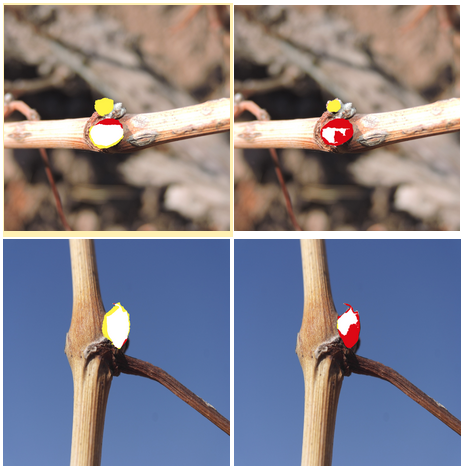
\includegraphics[width=12cm]{figures/buds.png}
	\caption{Intersección, segmentación y ground truth son blanco, amarillo y rojo respectivamente. Arquitectura 32s, Izquierda $\tau=0.5$, Derecha $\tau=0.9$}
	\label{fig:Fig1.3.1}
\end{figure}

Observando los resultados de Sliding Windows (Fig. 1.1.2), se mantiene siempre un alto recall pero con una precision de cómo mucho $0.4$ a $\nu=4$. Esto sucede porque el clasificador SVM de precision y recall $0.9$ aprox, está trabajando sobre un conjunto de patches desbalanceado al segmentar la imagen completa, por lo que existen muchos más patches negativos que positivos, aumentando la cantidad de falsos positivos. 
Vemos que las mejores variantes a $\nu=4$ son aquellas que tienen un tamaño de ventana que implica un overlap mínimo del tamaño de una yema promedio, esto es por ejemplo la 400 o 600 generan como mínimo una zona de overlap 200/300 píxeles, el cual es el tamaño promedio de una yema en el dataset original (248px) (para FCN se re-escalan a un tamaño menor respetando relación aspecto por limitaciones de hardware). A thresholds menores, las variantes con mayor tamaño de ventana (i.e 800, 900 o 1000px) reducen en gran medida los falsos positivos ya que la cantidad de zonas de overlap posibles son menos a medida que la ventana más grande es.

A la luz de los resultados obtenidos concluimos que FCN resulta superadora en resultados de localización ya que ninguna variante de SW supera los resultados de FCN, validando nuestra hipótesis que mediante un enfoque basado en Deep Learning se pueden conseguir resultados de detección superadores al estado del arte.

\subsection{4.1. Segmentación}
Ahora procedemos a analizar los resultados obtenidos en términos de métricas de segmentación, mediante las cuales podremos evaluar distintos aspectos sobre las segmentaciones producidas por FCN.

Los resultados de Precision y Recall de segmentación en la Figura 1.2.2, nos muestran resultados positivos respecto a la capacidad de FCN de poder segmentar correctamente la yema presente en la escena, con un $20\%$ de píxeles mal clasificados como yema (False Positive) y $20\%$ de pixeles en promedio que no son comprendidos (False Negative) en el componente más cercano al centro ground truth. Esto es especialmente positivo para aplicaciones donde se tenga que obtener una segmentación precisa de la instancia de yema, cómo puede ser fenotipado. 

La Figura 1.2.5 nos muestra una perspectiva interesante respecto a las características de los componentes generados para una escena. La tabla nos muestra el componente más grande y que en promedio resulta teniendo casi la totalidad del área de segmentación ($> 90\%$) es el componente que de hecho es el más cercano y a la vez intersecta a la yema verdadera. Esto es un aspecto que resulta muy positivo ya que debido a que las yemas presentes en una escena tienen cierto tamaño relativamente uniforme, es decir no existe una yema 100 veces más pequeña que otra, independientemente de la escala, podemos evaluar los componentes según su porcentaje de área relativa a todos los componentes que conforman la segmentación. De esta manera podemos plantear post-procesamientos donde se evalúe este parámetro (Área relativa de segmentación), permitiendo diferenciar componentes de muy poca área relativa que pueden ser considerados ruido de la segmentación.

\subsection{4.3. Localización}
La distancia promedio de los componentes generados por FCN son de gran importancia ya que se logra obtener detecciones donde la distancia en promedio no es mayor a un diámetro de yema. Esto es de especial utilidad para aplicaciones en las que la localización en el espacio de cada instancia sea relevante, como por ejemplo el seguimiento del desarrollo del viñedo donde se releva continuamente al viñedo y se necesita identificar en el espacio a cada yema. Debido a que la misma definición de True Positive implica que el componente debe estar cerca de la yema, evaluamos la distancia de aquellos componentes False Positive que se encuentran en escenas del conjunto de test donde no exista un True Positive. Este caso no se dio para la variante 8s y se dio solo una vez en el caso de las otras dos variantes. Donde para la 16s resultaron 1 false positive de distancia normalizada $0.73$ y para 32s 2 false positives cuya distancia normalizada fue de $0.44$.

Analizando los distintos resultados sistemáticos presentados en conjunto, vemos que cuando el enfoque basado en redes neuronales detecta una yema, este componente segmenta a la yema verdadera correctamente en un $60\%$ en promedio, a una distancia promedio entre centros de masa de medio diámetro de yema; y a su vez este componente,en promedio, es el de mayor área relativa a la segmentación total por lo que los demás componentes, falsos positivos, son de tamaño mucho menor.

A la luz de los resultados concluimos que el enfoque basado en redes completamente convolucionales se prueba cómo un enfoque efectivo para poder detectar yemas de vid en condiciones naturales de campo, y a su vez las detecciones producidas por la red pueden ser útiles para distintas otras aplicaciones donde la forma y posición de la yema tengan relevancia.

section{5. Discusión}

En esta sección se discuten los resultados obtenidos para la detección de yemas de vid y su impacto en la medición autónoma de variables vitícolas de interés, examinando sus  alcances y limitaciones desde un punto de vista práctico. Para esto se toman las variables de la Tabla 1 presentada en la introducción y se analiza individualmente el impacto de estos resultados para una de ellas.

Conteo de yemas
Clasificación del tipo de yema
Etapa de desarrollo de la yema
Longitud entre nudos (por detección de yemas)
Tamaño de yema (área o volumen)
Seguimiento del desarrollo de la yema
Incidencia de luz solar recibida por la yema
Poda de vid autónoma
Fenotipado
Reconstrucción 3D de la estructura de la planta y sus yemas.

IDEA: discutir las posibilidades de medición de varaibles real time


%#######################################################################
%#######################################################################
\section{Conclusions}

TODO: Conclusions

\section*{Acknowledgments}

Tal vez a alguien.

\section*{References}
\bibliography{2020-DeepBudDetection-CEA}

\end{document}